\documentclass[11pt]{article}
\usepackage{amsmath, fullpage, parskip, graphicx}

\begin{document}
\title{DS Coursework}
\author{Jacob Essex \\ s1040340}
\date{}
\maketitle

\subsection*{Q1}

I assume that the starting time $(0,0)$ is some point before either of the first events for $p_1$ or $p_2$ occur. This is slightly more general than the notation used in some of the slides in which it is assumed that both of the first events have occurred. Should this actually be what is wanted then as the below graph is more general the point at which the first two events have occurred is $(1,1)$

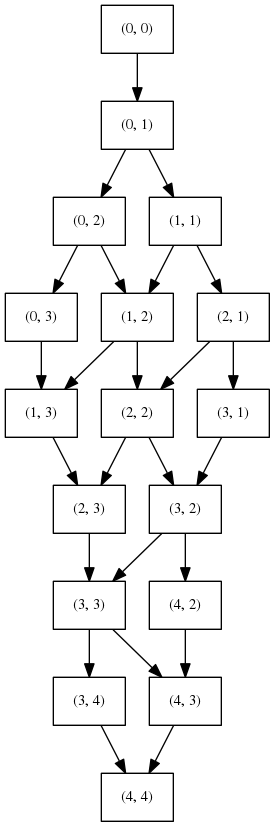
\includegraphics[width=0.25\textwidth]{q1_theory.png}


\subsection*{Q2}
To avoid starvation an algorithm needs to be fair (i.e. requests for a lock are honored in the order that they are made). This prevents starvation. A system that is liable to have starvation is one that always grants the request of the most recent request for a mutex over that of older requests.

\subsection*{Q3}

The response data is of fixed size and is represented using the following tuple
$$
(\text{sum of all p.f seen}, \text{max of all p.f seen}, \text{number of processors seen})
$$
The algorithm is as follows:

The root node $r$ sends a request to all of its children in the tree $T$ for the data. All children then send the request onwards to their children. This happens recursively and eventually  message has will propagate to all nodes. This takes $O(n)$ time as the message is a of a fixed length and in the worst case the tree is a list where each node has $0$ or $1$ children.

When a leaf node receives the request for the data it then sends $(p.f, p.f, 1)$ to its parent node.

For a node $p$, such that $p \neq r$, on receipt of data $(sum_i, max_i, count_i)$ from all its $n$ children, the node $p$ sends sends the following data to its parents 
$$
(p.f + \sum_{i=0}^n  sum_i, \text{MAX}(p.f, max_1, max_2, ... max_n), 1 + \sum_i^n count_i)
$$

For the node $r$ on receipt of data from all its $n$ children, $r$ does the same calculation as above:
$$(r.f + \sum_{i=0}^n  sum_i, \text{MAX}(r.f, max_1, max_2, ... max_n), 1 + \sum_i^n count_i)$$

So it then holds hold $(\text{sum}, \text{max}, \text{count})$.  It then preforms the following operation on its tuple to product a new tuple 
$$\text{result} = (\text{avg}, \text{max}) = (\text{sum/count}, \text{max})$$

This new tuple is the required result.

The response message length is also fixed, so the cost of sending a message is fixed.
Again in the worst case, the minimum spanning tree represents a list of processors so in this case $O(n)$ messages need to be sent sequentially taking $O(n)$ time.

In total the time taken for this algorithm is $O(n) + O(n) = O(n)$

\subsection*{Q4}
The diameter of the network is defined by the longest shortest path. In the case
the diameter of the weighted graph this is:
$d \rightarrow h \rightarrow l \rightarrow m$

If each edge had a weight of 1 then the following paths of cost 5 would realise this:
$ e \rightarrow a \rightarrow c \rightarrow g \rightarrow l \rightarrow m$ and
$e \rightarrow a \rightarrow c \rightarrow f \rightarrow i \rightarrow k$

Of course in both cases as the graph is undirected the reverse paths would also give the same results

\end{document}
